\documentclass[12pt]{article}
\usepackage[paperwidth=36in,paperheight=24in,margin=0in]{geometry}
\usepackage[T1]{fontenc}
\usepackage{lmodern,amsmath,amssymb,bm,microtype,tikz,xcolor}
\usetikzlibrary{arrows.meta,calc,decorations.markings}
\pagestyle{empty}
\setlength{\parindent}{0pt}
\definecolor{navy}{HTML}{142D49}
\definecolor{teal}{HTML}{007D88}
\definecolor{amber}{HTML}{D59421}
\definecolor{ink}{HTML}{26394F}
\definecolor{paper}{HTML}{F1F5F8}
\definecolor{linegray}{HTML}{D8E2EA}
\definecolor{softteal}{HTML}{E8F4F3}
\definecolor{softamber}{HTML}{FFF4DE}
\newcommand{\dd}{\,\mathrm d}
\newcommand{\R}{\mathbb R}
\newcommand{\Z}{\mathbb Z}
\newcommand{\CC}{\mathbb C}
\newcommand{\bodyfont}{\fontsize{23.2}{29.1}\selectfont\raggedright}
\newcommand{\smallbody}{\fontsize{20.6}{25.8}\selectfont\raggedright}
\newcommand{\status}[2]{\textcolor{#1}{\fontsize{15.5}{18}\selectfont\bfseries #2}}
\newcommand{\panel}[7]{%
  \draw[rounded corners=0.12in,fill=white,draw=linegray,line width=1.1pt]
    (#1,#2) rectangle ++(11.4,5.7);
  \draw[#5,line width=5pt,line cap=round]
    ($(#1,#2)+(0.24,0.15)$) -- ++(10.92,0);
  \node[anchor=north west,inner sep=0,text=navy,text width=10.7in]
    at ($(#1,#2)+(0.34,0.43)$)
    {\fontsize{42}{49}\selectfont\bfseries\textcolor{#5}{#3}\quad #4};
  \node[anchor=north east,inner sep=0] at ($(#1,#2)+(11.03,0.23)$) {\status{#5}{#6}};
  \draw[linegray,line width=0.9pt] ($(#1,#2)+(0.34,1.04)$) -- ++(10.72,0);
  \node[anchor=north west,inner sep=0,text=ink,text width=10.7in]
    at ($(#1,#2)+(0.35,1.23)$)
    {\bodyfont #7};
}
\begin{document}
\null
\begin{tikzpicture}[remember picture,overlay]
\begin{scope}[shift={(current page.north west)},x=1in,y=-1in]
\fill[paper] (0,0) rectangle (36,24);
\fill[navy] (0,0) rectangle (36,2.35);
\node[anchor=north west,inner sep=0,text=white] at (0.58,0.40)
  {\fontsize{70}{77}\selectfont\bfseries ZETA VORTEX FIELDS};
\node[anchor=north west,inner sep=0,text=white] at (0.63,1.48)
  {\fontsize{35.5}{43}\selectfont Bridge shear, modular kernels, and the open global positivity step};
\node[anchor=north east,inner sep=0,text=white,align=right] at (35.4,0.51)
  {\fontsize{26}{32}\selectfont A technical research map\\[0.09in]
   \fontsize{22}{29}\selectfont Exact identities \textcolor{teal!35!white}{\(\bullet\)}\quad
   \textcolor{amber!55!white}{open theorem} \(\bullet\)\quad conditional conclusion};
\node[anchor=north east,inner sep=0,text=white!75] at (35.4,1.64)
  {\fontsize{19}{23}\selectfont 36 $\times$ 24 inches\quad$|$\quad vector mathematics\quad$|$\quad read down each column};

\node[anchor=west,inner sep=0,text=navy] at (0.6,2.69)
  {\fontsize{23}{27}\selectfont\bfseries 1--3\quad GEOMETRY AND MODULAR INPUT};
\node[anchor=west,inner sep=0,text=navy] at (12.35,2.69)
  {\fontsize{23}{27}\selectfont\bfseries 4--6\quad EXACT KERNEL IDENTITIES};
\node[anchor=west,inner sep=0,text=navy] at (24.1,2.69)
  {\fontsize{23}{27}\selectfont\bfseries 7--9\quad GLOBAL CLAIM AND LIMITS};

% COLUMN ONE: input and geometry.
\panel{0.55}{3.02}{1}{Complex zeros as vortices}{teal}{ESTABLISHED}{%
\(F(z)=\xi(\tfrac12+z),\quad z=x+it,\qquad \Xi(t)=F(it).\)
\vspace{0.09in}
\[
 \mathbf V=\nabla\arg F=J\nabla\log|F|,\qquad
 \mathbf V(z)=m\frac{J(z-z_0)}{|z-z_0|^2}+O(1).
\]
Here \(J\) rotates a vector by \(90^\circ\); \(z_0\) is a zero of multiplicity \(m\).
\vspace{0.08in}
\begin{center}
\begin{tikzpicture}[x=0.8in,y=0.72in,>=Stealth,font=\fontsize{19}{22}\selectfont]
  \fill[softteal,rounded corners=7pt] (-3.25,-0.95) rectangle (3.25,1.6);
  \draw[navy!45,dashed,line width=1.4pt] (-1.7,-0.65)--(-1.7,1.23);
  \draw[navy!45,dashed,line width=1.4pt] (1.7,-0.65)--(1.7,1.23);
  \draw[navy,line width=1.6pt,->] (0,-0.7)--(0,1.4) node[above] {\(t\)};
  \node[below] at (-1.7,-0.66) {\(x=-a\)};
  \node[below] at (0,-0.66) {\(x=0\)};
  \node[below] at (1.7,-0.66) {\(x=a\)};
  \draw[amber,line width=3pt,<->] (-1.7,0.77)--(1.7,0.77);
  \node[fill=softteal,inner sep=3pt,text=navy] at (0,1.1) {bridge across the twin rails};
  \foreach \yy in {-0.25,0.36}{
    \fill[teal] (0,\yy) circle (3.2pt);
    \draw[teal,line width=1.5pt,->] (0.25,\yy) arc[start angle=0,end angle=290,x radius=0.25,y radius=0.25];
  }
  \node[text=teal,align=left] at (2.6,0.07) {local\\ circulation};
  \node[text=navy!70] at (-2.55,0.15) {schematic};
\end{tikzpicture}
\end{center}
}

\panel{0.55}{9.07}{2}{The actual shifted bridge}{teal}{ESTABLISHED}{%
\[
 E_a(z)=\Xi(z+ia)=A_a(z)-iB_a(z),\qquad a>0.
\]
\vspace{-0.10in}
\[
 \begin{aligned}
 A_a(t)&=\int_0^\infty\psi(u)\cosh(au)\cos(tu)\dd u,\\
 B_a(t)&=\int_0^\infty\psi(u)\sinh(au)\sin(tu)\dd u.
 \end{aligned}
\]
\vspace{-0.04in}
\[
 H(a,t)=|\Xi(t+ia)|^2=A_a(t)^2+B_a(t)^2.
\]
\begin{center}
\fcolorbox{teal}{softteal}{\parbox{9.55in}{\centering\vspace{0.08in}
\(\displaystyle W_a(t)=A_aB_a'-A_a'B_a=\frac12\,\partial_aH(a,t).\)
\vspace{0.08in}}}
\end{center}
The primes differentiate \(t\). The target is the sign of this \emph{complete} shear at every height and shift.
}

\panel{0.55}{15.12}{3}{The full modular profile}{teal}{ESTABLISHED}{%
\[
 \psi(u)=\sum_{n=1}^\infty
 \left(8\pi^2n^4e^{9u/2}-12\pi n^2e^{5u/2}\right)
 e^{-\pi n^2e^{2u}}.
\]
\[
 \Xi(z)=\int_0^\infty\psi(u)\cos(zu)\dd u,
 \qquad \psi(u)=\psi(-u)>0.
\]
\begin{center}
\fcolorbox{teal}{softteal}{\parbox{9.55in}{\centering\vspace{0.06in}
\(\displaystyle \psi^{(2j+1)}(0)=0\quad(j=0,1,2,\ldots).\)
\vspace{0.06in}}}
\end{center}
These exact odd-jet cancellations use the complete theta sum. For a raw finite theta cutoff, \(d_N=\psi_N'(0)>0\), and
\[
 W_{a,N}(t)=-\frac{2a\,d_N^2}{t^6}+O(t^{-8})<0
 \quad\text{eventually}.
\]
\smallbody A finite cutoff can create a false sign obstruction. An even approximation still needs a separate positivity proof.
}

% COLUMN TWO: exact transforms.
\panel{12.3}{3.02}{4}{The complete shear kernel}{teal}{ESTABLISHED}{%
\[
 \boxed{\displaystyle
 C_a(v)=\int_0^\infty h\sinh(2ah)
          \psi(h-v)\psi(h+v)\dd h.}
\]
\vspace{0.04in}
\[
 \widehat C_a(k)=\int_{\R} C_a(v)e^{-ikv}\dd v,
 \qquad \boxed{\widehat C_a(2t)=W_a(t).}
\]
\vspace{0.02in}
\begin{center}

\begin{tikzpicture}[x=1in,y=1in,>=Stealth,font=\fontsize{24}{28}\selectfont]
 \node[draw=teal,fill=softteal,rounded corners=8pt,minimum width=3.65in,minimum height=0.8in,align=center] (a) at (0,0)
    {\(C_a(v)>0\)\\ pointwise};
 \node[draw=amber,fill=softamber,rounded corners=8pt,minimum width=3.65in,minimum height=0.8in,align=center] (b) at (5.5,0)
    {\(\widehat C_a(k)\ge0\)?\\ every frequency};
 \draw[navy,line width=2pt,->] (a)--node[above,font=\fontsize{18}{22}\selectfont]{Fourier}(b);
\end{tikzpicture}
\end{center}
\vspace{0.03in}
The integrand is nonnegative. That establishes pointwise positivity, but Fourier positivity requires control of all oscillatory cancellations.
}

\panel{12.3}{9.07}{5}{A positive autocorrelation}{teal}{ESTABLISHED}{%
\[
 f_a(u)=e^{au}\psi(u),\qquad
 R_a(v)=\int_{\R} f_a(h-v)f_a(h+v)\dd h.
\]
\[
 R_a\ \text{is positive definite},\qquad
 \widehat R_a(2t)=2|\Xi(t+ia)|^2=2H(a,t).
\]
\begin{center}
\fcolorbox{teal}{softteal}{\parbox{9.55in}{\centering\vspace{0.10in}
\(\displaystyle C_a(v)=\frac14\,\partial_aR_a(v).\)
\vspace{0.10in}}}
\end{center}
\vspace{0.02in}
This is an exact positive factorization of \(R_a\). To obtain the required shear inequality, its derivative must also be positive definite.
\vspace{0.10in}
\begin{center}\textcolor{amber}{\bfseries Positive operators need not have positive derivatives.}\end{center}
}

\panel{12.3}{15.12}{6}{Epstein differential identity}{teal}{EXACT IDENTITY}{%
\(p=a+\tfrac12,\quad D_v=\partial/\partial v.\) Define the completed rectangular Epstein zeta function
\[
 E^*(p,v)=\pi^{-p}\Gamma(p)
 \sideset{}{'}\sum_{(m,n)\in\Z^2}
 \left(n^2e^{-2v}+m^2e^{2v}\right)^{-p}.
\]
\vspace{-0.07in}
\smallbody The lattice series requires \(\Re p>1\). Use its meromorphic continuation for \(0<a<\tfrac12\).
\bodyfont
\[
 \mathcal L_a=\big[D_v^2-(2a-1)^2\big]\big[D_v^2-(2a+1)^2\big].
\]
\vspace{-0.11in}
\[
 R_a=\frac1{32}\mathcal L_a E^*(a+\tfrac12,v),\qquad
 \boxed{C_a=\frac1{128}\partial_a\!\left[\mathcal L_a E^*\right].}
\]
\smallbody The operator cancels the poles at \(p=0,1\). The identity reorganizes the complete modular sum; it does not establish the sign of the derivative.
}

% COLUMN THREE: the precise open step, consequence, and geometric limits.
\panel{24.05}{3.02}{7}{The missing global theorem}{amber}{OPEN}{%
Prove, for every \(0<a<\tfrac12\), every finite real node set, and every vector of complex coefficients,
\[
 \boxed{\displaystyle
 \sum_{j,k}\overline{c_j}c_k\,C_a(v_j-v_k)\ge0.}
\]
Equivalently, prove Loewner monotonicity of the autocorrelation kernels:
\[
 R_b-R_a\succeq0\qquad(0<a<b<\tfrac12).
\]
In the Epstein representation, the precise target is
\[
 \partial_a\!\left[\mathcal L_a E^*(a+\tfrac12,\cdot)\right]\succeq0.
\]
\begin{center}\textcolor{amber!85!black}{\bfseries No factorization or positivity theorem for this derivative is established here.}\end{center}
}

\panel{24.05}{9.07}{8}{How positivity traps a zero}{amber}{CONDITIONAL}{%
If Panel 7 holds, then \(W_a(t)\ge0\) for all real \(t\) and \(0<a<\tfrac12\). Suppose an off-line zero exists:
\[
 \Xi(\gamma+ib)=0,\quad 0<b<\tfrac12,\qquad
 \Xi(z)=c(z-\gamma-ib)^m+\cdots.
\]
Evaluate just below it, at \(a=b-\varepsilon\):
\[
 \boxed{\displaystyle
 W_{b-\varepsilon}(\gamma)
   =-m|c|^2\varepsilon^{2m-1}+O(\varepsilon^{2m})<0.}
\]
This contradicts the global inequality. Reflection handles the opposite side of the critical line.
\par\vspace{0.08in}
\makebox[\linewidth][c]{\textcolor{navy}{\fontsize{36}{42}\selectfont\bfseries Global kernel positivity\quad\(\Longrightarrow\)\quad RH}}
\par\vspace{0.08in}
\smallbody The implication is proved; its positivity premise in Panel 7 remains open.
}

\panel{24.05}{15.12}{9}{The sphere shows the limit}{navy}{GEOMETRY ONLY}{%
\begin{minipage}[t]{4.20in}
\vspace{0pt}
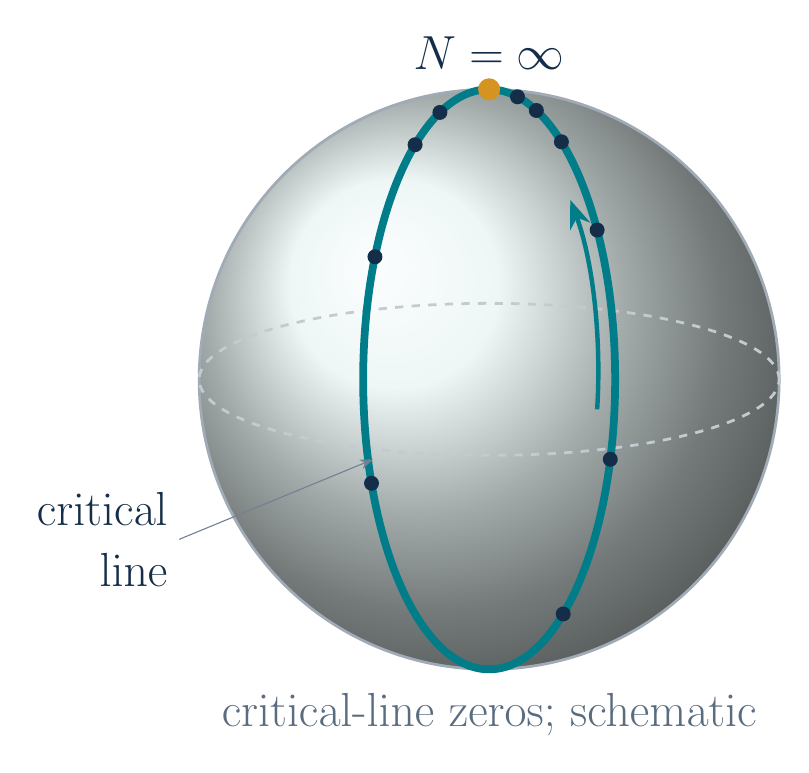
\begin{tikzpicture}[x=1in,y=1in,>=Stealth,font=\fontsize{18}{22}\selectfont]
 \shade[ball color=softteal] (0,0) circle (1.45);
 \draw[navy!40,line width=1pt] (0,0) circle (1.45);
 \draw[navy!25,dashed,line width=1pt] (0,0) ellipse (1.45 and 0.38);
 \draw[teal,line width=2.8pt] (0,0) ellipse (0.63 and 1.45);
 \draw[teal,line width=1.6pt,->] (0.54,-0.15) arc[start angle=-8,end angle=40,x radius=0.60,y radius=1.34];
 \foreach \ang in {-54,-16,31,55,68,77}{
  \fill[navy] ({0.63*cos(\ang)},{1.45*sin(\ang)}) circle (2.7pt);
 }
 \foreach \ang in {113,126,155,201}{
  \fill[navy] ({0.63*cos(\ang)},{1.45*sin(\ang)}) circle (2.7pt);
 }
 \fill[amber] (0,1.45) circle (4pt);
 \node[above,text=navy] at (0,1.5) {\(N=\infty\)};
 \draw[navy!60,->] (-1.55,-0.8)--(-0.58,-0.4);
 \node[anchor=east,align=right,text=navy] at (-1.56,-0.8) {critical\\ line};
 \node[below,text=navy!70,font=\fontsize{16}{20}\selectfont] at (0,-1.52) {critical-line zeros; schematic};
\end{tikzpicture}
\end{minipage}\hfill
\begin{minipage}[t]{6.12in}
\vspace{0.04in}
Stereographic coordinates place \(x=0\) on a great circle through infinity:
\[
 S(x+it)=\frac{(2x,\,2t,\,x^2+t^2-1)}{1+x^2+t^2}.
\]
Both ends of the infinite critical line meet \(N\). Infinitely many zeros accumulate there.\par
\vspace{0.12in}
The phase field is singular at the zeros and has no smooth global extension at \(N\). The hairy-ball theorem does not locate the zeros on the critical line.
\end{minipage}
}

% In-column progression indicators.
\foreach \xx in {6.25,18.0,29.75}{
 \draw[navy!45,line width=2pt,-{Stealth[length=9pt,width=8pt]}] (\xx,8.77)--(\xx,9.01);
 \draw[navy!45,line width=2pt,-{Stealth[length=9pt,width=8pt]}] (\xx,14.82)--(\xx,15.06);
}

% Research targets and bibliographic context.
\draw[navy!25,line width=1pt] (0.60,21.15)--(35.4,21.15);
\node[anchor=north west,inner sep=0,text=navy] at (0.62,21.36)
 {\fontsize{26}{31}\selectfont\bfseries THREE CONCRETE RESEARCH TARGETS};
\node[anchor=north west,inner sep=0,text=ink,text width=10.65in] at (0.64,21.94)
 {\fontsize{23}{28}\selectfont\textcolor{teal}{\bfseries 01}\quad Factor the \(a\)-derivative into positive quadratic forms while retaining the complete modular sum.};
\node[anchor=north west,inner sep=0,text=ink,text width=10.65in] at (12.37,21.94)
 {\fontsize{23}{28}\selectfont\textcolor{teal}{\bfseries 02}\quad Find a theta-specific positivity mechanism for the entire associated-kernel hierarchy.};
\node[anchor=north west,inner sep=0,text=ink,text width=10.65in] at (24.1,21.94)
 {\fontsize{23}{28}\selectfont\textcolor{teal}{\bfseries 03}\quad Control every interval and limiting domain in an arithmetic canonical-system construction.};
\node[anchor=south west,inner sep=0,text=navy!75,text width=34.7in] at (0.64,23.59)
 {\fontsize{17.7}{21.8}\selectfont
 \textbf{Background:} G. Csordas, \emph{Fourier Transforms of Positive Definite Kernels and the Riemann $\xi$-Function} (2015);
 J. C. Lagarias, \emph{On a positivity property of the Riemann $\xi$-function} (1999), correction (2005);
 R. L. Hudson, \emph{When is the Wigner quasi-probability density non-negative?} (1974).
 \quad\textbf{Status:} an exact research reduction with the global positivity step explicitly open.};
\end{scope}
\end{tikzpicture}
\end{document}
